\documentclass[12pt,a4paper]{article}
\usepackage[utf8]{inputenc}
\usepackage[spanish,es-tabla,es-noquoting]{babel}
\usepackage{geometry}
\usepackage{graphicx}
\usepackage{multirow}
\usepackage{tabularx}
\usepackage{longtable}
\usepackage{float}
\usepackage{amsmath}
\usepackage{amssymb}
\usepackage{mathptmx}
\usepackage{fancyhdr}
\usepackage{array}
\usepackage[table]{xcolor}
\usepackage{titlesec}
\usepackage{setspace}
\usepackage{microtype}
\usepackage{lastpage}
\usepackage{booktabs}
\usepackage{enumitem}
\usepackage{hyperref}
\usepackage{listings}

\hypersetup{
    colorlinks=true,
    linkcolor=black,
    citecolor=blue!70!black,
    urlcolor=blue!70!black
}

\graphicspath{{images/}{../images/}{./}}

\geometry{
    top=4.7cm,
    bottom=2.5cm,
    left=2.5cm,
    right=2.5cm,
    headheight=3.9cm,
    headsep=0.4cm
}

\setstretch{1.15}
\setlength{\parindent}{0pt}
\setlength{\parskip}{0.45em}
\setlength{\tabcolsep}{4pt}

\titleformat{\section}
  {\normalfont\fontsize{12}{14.5}\bfseries}{\thesection.}{0.6em}{\uppercase}
\titlespacing*{\section}
  {0pt}{1.8ex plus 0.4ex minus 0.2ex}{0.6ex plus 0.2ex}

\titleformat{\subsection}
  {\normalfont\fontsize{11.5}{13.5}\bfseries}{\thesubsection.}{0.5em}{}
\titlespacing*{\subsection}
  {0pt}{1.4ex plus 0.3ex minus 0.1ex}{0.4ex plus 0.1ex}

\titleformat{\subsubsection}
  {\normalfont\fontsize{10.5}{12.5}\bfseries\itshape}{\thesubsubsection.}{0.4em}{}
\titlespacing*{\subsubsection}
  {0pt}{1.1ex plus 0.2ex minus 0.1ex}{0.3ex plus 0.1ex}

\newcolumntype{Y}{>{\centering\arraybackslash}X}
\newcolumntype{L}{>{\raggedright\arraybackslash}X}
\newcolumntype{C}{>{\centering\arraybackslash}X}

\definecolor{headerred}{RGB}{180, 0, 0}
\definecolor{darkred}{RGB}{140, 0, 0}
\definecolor{lightgraybg}{RGB}{248, 248, 248}
\definecolor{tableheader}{RGB}{232, 238, 246}
\definecolor{navyheader}{RGB}{0, 52, 94}

\newcommand{\docCodigo}{TI-SIGE-ENT-F3-012}
\newcommand{\docVersion}{1.0}
\newcommand{\docProceso}{INGENIERÍA DE SOFTWARE / PROCESAMIENTO DE LENGUAJE NATURAL}
\newcommand{\docElaboracion}{05/10/2026}
\newcommand{\docRevision}{05/10/2026}
\newcommand{\docTitulo}{INTEGRACIÓN DE CAPA DE IA LOCAL: SERVICIO LANGUAGETOOL EN DOCKER}
\newcommand{\docOrganizacion}{FACULTAD DE INGENIERÍA EN SISTEMAS, ELECTRÓNICA E INDUSTRIAL}
\newcommand{\docSubOrganizacion}{CARRERA DE INGENIERÍA DE SOFTWARE}

\newcommand{\encabezadofrecuente}{%
    \renewcommand{\arraystretch}{1.15}%
    \noindent\makebox[\textwidth][c]{%
    \begin{tabularx}{\textwidth}{|>{\centering\arraybackslash}m{2.8cm}|Y|>{\centering\arraybackslash}m{4.8cm}|}
        \hline
        \multirow{4}{2.8cm}{\centering\raisebox{-1.15cm}{
\includegraphics[width=2.5cm,height=2.0cm,keepaspectratio]{images/logo.png}}}
        & \textbf{\fontsize{9}{11}\selectfont \docOrganizacion} 
        & \textbf{\fontsize{8}{10}\selectfont CÓDIGO:} \fontsize{8}{10}\selectfont \docCodigo \\
        \cline{3-3}
        & \textbf{\fontsize{8.5}{10.5}\selectfont \docSubOrganizacion} 
        & \textbf{\fontsize{8}{10}\selectfont VERSIÓN:} \fontsize{8}{10}\selectfont \docVersion \\
        \cline{2-3}
        & \textbf{\fontsize{8}{10}\selectfont PROCESO:} \fontsize{8}{10}\selectfont \docProceso 
        & \textbf{\fontsize{8}{10}\selectfont ELABORACIÓN:} \fontsize{8}{10}\selectfont \docElaboracion \\
        \cline{2-3}
        & \textbf{\fontsize{8.5}{10.5}\selectfont \docTitulo} 
        & \textbf{\fontsize{8}{10}\selectfont ÚLTIMA REVISIÓN:} \fontsize{8}{10}\selectfont \docRevision \\
        \hline
    \end{tabularx}%
    }%
}

\pagestyle{fancy}
\fancyhf{}
\fancyhead[C]{\encabezadofrecuente}
\fancyfoot[C]{\fontsize{10}{12}\selectfont Página \thepage\ de \pageref{LastPage}}
\renewcommand{\headrulewidth}{0pt}

\lstset{
  basicstyle=\ttfamily\scriptsize,
  backgroundcolor=\color{lightgraybg},
  frame=single,
  breaklines=true,
  tabsize=2,
  showstringspaces=false
}

\begin{document}

\noindent{\fontsize{10.5}{12.5}\selectfont \textbf{Integrantes:} Heidi Villavicencio \quad$\vert$\quad Steeven Toala \quad$\vert$\quad Nixon Hurtado \quad$\vert$\quad Andrea Vásquez}

\vspace{0.25cm}

\section{Título}
\textbf{Denominación del Entregable:} Integración de la Capa de Inteligencia Local: Servicio LanguageTool en Docker para Corrección Gramatical y Estilística -- Código EDT: 3.12 (Fase 3: Desarrollo Iterativo Core).

\section{Introducción}
La calidad de los Planes de Trabajo e Informes Semestrales en la FISEI UTA no se circunscribe únicamente al cumplimiento cuantitativo de horas; requiere además un estándar riguroso de redacción formal, concordancia gramatical y precisión ortográfica acorde a la documentación institucional auditada por el CACES y el Sistema de Gestión de Calidad (SGC).

Históricamente, los documentos presentados evidenciaban erratas tipográficas y discordancias estilísticas. Para solucionar esta problemática sin comprometer la confidencialidad de la información institucional mediante APIs públicas en la nube, se integró un microservicio local de \textbf{LanguageTool} contenerizado en Docker. Este servicio opera como un componente analítico desacoplado, proveyendo sugerencias en tiempo real directamente sobre el editor de texto enriquecido TipTap.

\section{Objetivo}

\subsection{Objetivo General}
Desplegar e integrar un microservicio local de procesamiento de lenguaje natural basado en LanguageTool mediante Docker Compose, habilitando la verificación ortográfica, gramatical y estilística en tiempo real para la redacción de planes e informes académicos en SIGE.

\subsection{Objetivos Específicos}
\begin{itemize}[leftmargin=1.5em, itemsep=1.5pt]
    \item Configurar el contenedor oficial de LanguageTool optimizado para idioma español (\texttt{es-EC} / \texttt{es}) en la red local interna de Docker.
    \item Implementar el puente de comunicación en el backend Express y el hook de inspección con técnica \textit{debounce} en el frontend TipTap.
    \item Garantizar la soberanía de datos institucional bajo el estándar ISO/IEC 27001 evitando la transmisión de datos fuera del servidor local.
\end{itemize}

\section{Alcance}

\subsection{Límites de Implementación (In-Scope)}
\begin{itemize}[leftmargin=1.5em, itemsep=1.5pt]
    \item Despliegue del contenedor \texttt{erikvl87/languagetool} en puerto interno 8010.
    \item Análisis sintáctico y ortográfico de secciones textuales (Justificación, Objetivos, Conclusiones y Recomendaciones).
    \item Resaltado visual en el editor TipTap con marcas flotantes y lista de sugerencias de reemplazo.
\end{itemize}

\subsection{Exclusiones (Out-of-Scope)}
\begin{itemize}[leftmargin=1.5em, itemsep=1.5pt]
    \item Generación autónoma de texto (la corrección es supervisada; el docente decide si aplica la sugerencia).
    \item Corrección de datos numéricos o nombres propios específicos no contemplados en el diccionario de la lengua española.
\end{itemize}

\section{Definiciones}
\begin{itemize}[leftmargin=1.5em, itemsep=2pt]
    \item \textbf{LanguageTool:} Motor de código abierto para verificación gramatical, ortográfica y de estilo que analiza reglas sintácticas y contextos morfológicos.
    \item \textbf{Procesamiento Local (On-Premise):} Ejecución de modelos y servicios dentro de la infraestructura controlada de la institución, garantizando total privacidad.
    \item \textbf{Debounce:} Mecanismo de optimización en programación que retrasa la ejecución de una función de red hasta que el usuario haya dejado de escribir durante un umbral de milisegundos.
    \item \textbf{Soberanía de Datos:} Principio de seguridad de la información que impide la transferencia no autorizada de datos institucionales hacia servidores de terceros en el extranjero.
\end{itemize}

\section{Responsabilidades}
\begin{itemize}[leftmargin=1.5em, itemsep=2pt]
    \item \textbf{Analista de Requisitos / UI-UX (Heidi Villavicencio):} Relevamiento y modelado de necesidades, especificaciones funcionales, diseño de interfaces de usuario y verificación de usabilidad.
    \item \textbf{Líder de Proyecto / Arquitecto de Software (Steeven Toala):} Arquitectura de software, gobierno técnico, cumplimiento metodológico del cronograma y control de calidad integral.
    \item \textbf{Desarrollador Backend / DBA (Nixon Hurtado):} Modelo de base de datos PostgreSQL, persistencia de datos, seguridad por roles y reglas lógicas de validación.
    \item \textbf{Desarrolladora Frontend / QA (Andrea Vásquez):} Implementación de componentes React, manejo de estado global, integración de APIs y ejecución de pruebas de aceptación.
    \item \textbf{Docente Evaluador / Tutor (Ing. Paulo Torres, Mg.):} Dirección académica, asesoría metodológica, revisión de suficiencia técnica y validación institucional de los entregables.
\end{itemize}

\section{Normativa Legal y Técnica}
\begin{itemize}[leftmargin=1.5em, itemsep=2pt]
    \item \textbf{ISO/IEC 27001:2022 (Control 8.24):} Uso de criptografía y aislamiento de microservicios para resguardar la confidencialidad de la información.
    \item \textbf{ISO/IEC 25010 (Eficiencia de Desempeño y Usabilidad):} Respuestas de verificación con latencia inferior a 200 ms en red local.
    \item \textbf{Ley Orgánica de Protección de Datos Personales (LOPDP Ecuador):} Salvaguarda de los datos académicos y laborales del personal docente.
\end{itemize}

\section{Método, Políticas y Contenidos}
La integración técnica se diseñó bajo las siguientes políticas:
\begin{enumerate}[leftmargin=1.5em, itemsep=2pt]
    \item \textbf{Aislamiento de Red:} LanguageTool expone su API HTTP internamente hacia el backend Node.js, impidiendo consultas externas directas no autenticadas.
    \item \textbf{Políticas de Sobrecarga (Debounce de 750 ms):} El editor solo envía el payload de texto al transcurrir 750 ms de inactividad de teclado, evitando saturar la CPU del contenedor.
    \item \textbf{Caché de Verificación:} Párrafos idénticos no modificados se resuelven mediante almacenamiento temporal en memoria, optimizando recursos.
\end{enumerate}

\begin{figure}[htbp]
    \centering
    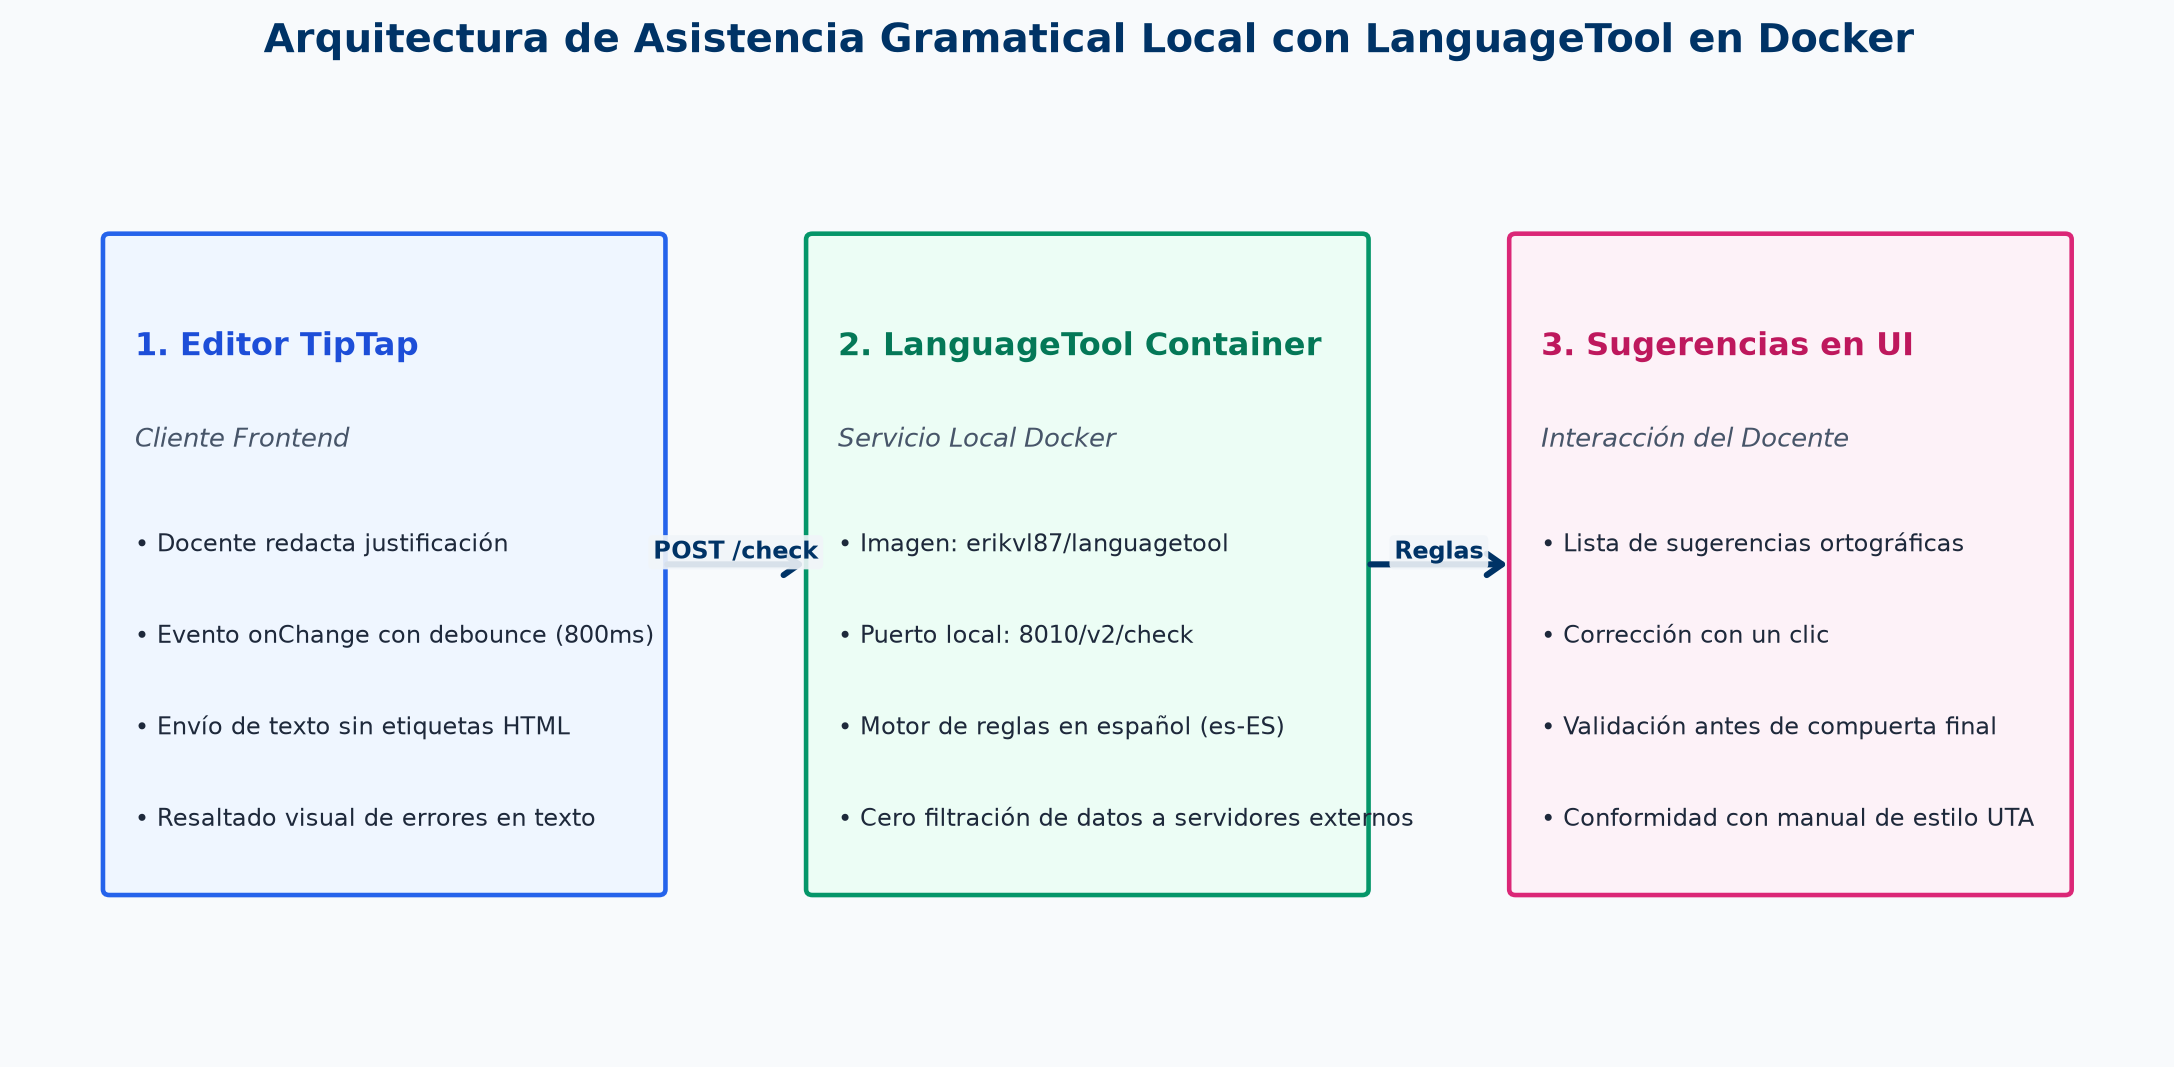
\includegraphics[width=0.92\textwidth,keepaspectratio]{images/f3_12_languagetool_docker.png}
    \caption{Arquitectura de Asistencia Gramatical Local con LanguageTool en Contenedor Docker.}
    \label{fig:docker_languagetool}
\end{figure}

\section{Descripción de actividades}

\subsection{Configuración en docker-compose.yml}
Se definió el servicio \texttt{languagetool} asignándole límites de memoria y reinicio automático:
\begin{lstlisting}[language=SQL]
  # Servicio local de LanguageTool en docker-compose.yml
  languagetool:
    image: erikvl87/languagetool:latest
    container_name: sige_languagetool
    restart: unless-stopped
    ports:
      - "8010:8010"
    environment:
      - EXTRA_OPTIONS=--config /config/server.properties
      - Java_Xms=512m
      - Java_Xmx=1024m
    networks:
      - sige-network
\end{lstlisting}

\subsection{Servicio de Comunicación Backend (languagetool.service.js)}
El backend implementa un cliente HTTP dedicado para enviar el texto al servicio:
\begin{lstlisting}
// backend/src/services/languagetool.service.js
const axios = require('axios');

const LANGUAGETOOL_URL = process.env.LANGUAGETOOL_URL || 'http://languagetool:8010/v2/check';

exports.checkText = async (text, language = 'es') => {
  if (!text || text.trim() === '') return { matches: [] };
  
  const params = new URLSearchParams();
  params.append('text', text);
  params.append('language', language);

  const response = await axios.post(LANGUAGETOOL_URL, params, {
    headers: { 'Content-Type': 'application/x-www-form-urlencoded' },
    timeout: 3000
  });

  return response.data;
};
\end{lstlisting}

\begin{figure}[htbp]
    \centering
    
\includegraphics[width=0.88\textwidth,keepaspectratio]{images/plan_page_2.png}
    \caption{Visualización de Correcciones Ortográficas y Gramaticales en el Editor TipTap de SIGE.}
    \label{fig:editor_languagetool_preview}
\end{figure}

\section{Firmas de Responsabilidad}

\noindent
\renewcommand{\arraystretch}{1.2}
\begin{tabularx}{\textwidth}{|>{\raggedright\arraybackslash}m{2.9cm}|>{\raggedright\arraybackslash}X|>{\centering\arraybackslash}m{4.6cm}|>{\centering\arraybackslash}m{2.3cm}|}
    \hline
    \rowcolor{tableheader}
    \textbf{ACCIÓN} & \textbf{NOMBRE Y CARGO} & \textbf{FIRMA} & \textbf{FECHA} \\
    \hline
    \textbf{Elaborado por:} & Heidi Villavicencio\newline Analista de Requisitos / UI-UX & \parbox[c]{4.4cm}{\centering\vspace{4pt}
\includegraphics[height=1.5cm,width=4.0cm,keepaspectratio]{images/firma_heidi.png}\vspace{4pt}} & 05/10/2026 \\
    \hline
    \textbf{Revisado por:} & Steeven Toala\newline Líder de Proyecto / Arquitecto & \parbox[c]{4.4cm}{\centering\vspace{4pt}
\includegraphics[height=1.5cm,width=4.0cm,keepaspectratio]{images/firma_steveen.png}\vspace{4pt}} & 05/10/2026 \\
    \hline
    \textbf{Aprobado por:} & Ing. Paulo Torres, Mg.\newline Docente Evaluador -- Gestión Proyectos & \parbox[c]{4.4cm}{\centering\vspace{8pt}\textbf{\textcolor{gray!80}{\scriptsize [ PENDIENTE DE APROBACIÓN ]}}\vspace{8pt}} & \textbf{\textcolor{gray!90}{Pendiente}} \\
    \hline
\end{tabularx}

\vspace{0.4cm}

\section{Control de Cambios}

\noindent
\renewcommand{\arraystretch}{1.2}
\begin{tabularx}{\textwidth}{|>{\hsize=0.45\hsize\centering\arraybackslash}X|>{\hsize=1.55\hsize\raggedright\arraybackslash}X|>{\hsize=1.2\hsize\raggedright\arraybackslash}X|>{\hsize=0.8\hsize\centering\arraybackslash}X|}
    \hline
    \rowcolor{tableheader}
    \textbf{Versión} & \textbf{Descripción del cambio} & \textbf{Responsable del cambio} & \textbf{Fecha de aprobación} \\
    \hline
    1.0 & Configuración y despliegue del contenedor Docker LanguageTool e integración con el editor de textos. & Andrea Vásquez / Nixon Hurtado & 05/10/2026 \\
    \hline
\end{tabularx}

\vspace{0.4cm}

\section{Anexos}

\subsection*{Anexo 1: Estructura del Objeto JSON de Sugerencias Retornado por LanguageTool}
\begin{lstlisting}[language=JavaScript]
{
  "software": { "name": "LanguageTool", "version": "6.4" },
  "language": { "name": "Spanish", "code": "es" },
  "matches": [
    {
      "message": "Posible error ortográfico o tipográfico.",
      "shortMessage": "Error ortográfico",
      "offset": 45,
      "length": 8,
      "replacements": [ { "value": "elaboró" }, { "value": "elabora" } ],
      "rule": { "id": "SPANISH_SPELLER_RULE", "description": "Corrector ortográfico" }
    }
  ]
}
\end{lstlisting}

\end{document}
